\section{Approach}
\label{sec:approach}

The DMAS solution we developped defines two agents, \emph{Package Agents} and
\emph{Truck Agents}. All Package Agents have a corresponding package and are
located on the pickup location of that package. Truck Agents control a
corresponding truck and move along with the truck. Both agents also own a
\emph{pheromone table}. These tables can hold multiple paths (list of Package
Agents in a certain order) and a corresponding pheromone (heuristic value).

\npar Package Agents and Truck Agents communicate with each other by sending
ants. These are a sort of smart messages.

\npar There is also a \emph{"forwarder"} placed in each delivery location of a
package. These \emph{"forwarders"} will send all received ants to the Package
Agent corresponding with the package for the local delivery location. Because of
their limited intelligence, forwarders are not considered to be agents.

\npar Like most DMAS based on ACO, three type of ants will be used. They will be
used in the following way:

\begin{description}
	\item[Feasability Ants] These ants will be periodically broadcasted
	over a certain radius from the Package Agents to the forwarders (delivery
	locations). Their main purpose is to inform other Package Agents wich Package
	Agents are in a certain radius near their delivery location.

	\item[Exploration Ants] These ants will be sent from the Truck Agents
	to discover and evaluate a path of Package Agents. They will update the
	pheromons table in the Package Agents during their return over the discovered
	path.
	
	\item[Intention Ants] These ants will be sent from the Truck Agents
	over the path of Package Agents that they are planning to follow. These ants
	will decrease the pheromone values for that path in the visited Package Agents
	in order to discourage other agents to follow this path.
\end{description}

\npar How agents find an optimal path by using the pheromones and communication
over ants is further explained in the following scenarios.

\subsection*{Scenario I: Broadcasting of Feasibility Ants}
\label{subsec:scenario1}
\npar \textit{Scenario I is illustrated in Figure \ref{Fig:scenario1}.}

\npar In this scenario Package Agent A (depicted as a brown box 'A') is added to the simulation. It will broadcast a Feasibility Ant \textit{$\rightarrow A$} in a certain radius to all forwarders (depicted as yellow flags). Forwarders C' and B' receive the feasibility ant and send it to their corresponding Package Agents C and B. These Package Agents now know in the future that package A is near after they are delivered. C and B will therefore add path \textit{$\rightarrow A$} to their tables with a default pheromone value, they will broadcast a new Feasibility Ant \textit{$\rightarrow CA$} and \textit{$\rightarrow BA$} respectively. Only forwarder F' receives the ant \textit{$\rightarrow BA$} this time and sends it to Package Agent F. Package agent F will add \textit{$\rightarrow BA$} to its pheromone table and broadcast a new Feasibility Ant again so the whole process can repeat itself. This goes on until the max number of hops (= number of broadcasts) is reached.

\npar For the classic PDP problem, a max number of hops of 1 is fine. Package Agents only need to know which other Package Agents are near their delivery location. Therefore only one broadcast is needed. Nevertheless could some extensions of PDP benefit from multiple hops (obligatory agents etc ...).

\subsection*{Scenario II: Sending of Exploration Ants}
\label{subsec:scenario2}
\npar \textit{Scenario II is illustrated in Figure \ref{Fig:scenario2}.}


\npar In this scenario, the Truck Agent is moving to Package Agent E to pick up the package. It sends an ExplorationAnt to Package Agent E to explore wich other packages he is able to pick up after he delivers package E. Package Agent E receives the ExplorationAnt and sees in his pheromone table that packages G and B are near the dellivery location of E. Scenario I (\ref{subsec:scenario1}) showed how these entries came into the pheromone table through Feasibility Ants. Package Agent E choses to send the Exploration Ant further to either \textit{$\rightarrow G$} or \textit{$\rightarrow B$}. The higher the pheromone value for a path the higher the chance that the path will be chosen. The pheromone value \textit{"evaporates"}  over time but returning Exploration Ants from that path can increase the pheromone value. The amount to increase depends on a heuristic function that takes several properties of the path into account, like the priority of the packages and the distance to the pickup location.

\npar PackageAgent E choses to send the Exploration Ant further to PackageAgent B, who in turn choses \textit{$\rightarrow A$} (using his pheromone table) to send it further to PackageAgent A. The Exploration Ant has reached its max number of hops and PackageAgent A send the ant back to B. In B, the ExplorationAnt will evaluates the path \textit{$\rightarrow A$} and increase its pheromone value before going back to E. In E, the ExplorationAnt will evaluates the path \textit{$\rightarrow B$} and increase its pheromone value before going back to Truck. At the truck the exploration ant will put the whole path \textit{$\rightarrow EBA$} in the pheromone table (if it was not already in there) and increase the pheromone value with the evauluated value for the whole path \textit{$\rightarrow EBA$}. 

\subsection*{Scenario III: Sending of Intention Ants}
\label{subsec:scenario3}
\npar \textit{Scenario II is illustrated in Figure \ref{Fig:scenario3}.}
\npar In this scenario the truck sends an Intention Path over the whole path of Package Agents that its planning to do. This path is the path with the highest corresponding pheromone value. Just as with pheromone tables for Package Agents do these pheromone values \textit{"evaporate"} in time. They get increased by returning Exploration Ants though.

\npar The path the truck is planning to do is \textit{$\rightarrow EGF$}. The truck sends an Intention Ant to Package Agent E. The Intention Ant will mark Package Agent E as "claimed by Truck X for time Y". This means that this Package Agent will no longer contribute pheromones for other trucks in the heuristic function to evaluate a path. If after a time Y no new Intention ant has reclaimed the Package Agent for truck X, the claim will expire and the PackageAgent will again contribute pheromones for other Trucks.

\npar After Package Agent E, the Intention Ant is send to Package Agents G and then F to do the same there. After Package Agent F then Intention Ant is send back to the truck to evaluate the whole path again (in the same way as an Exploration Ant). This is not necessary though.





 for  decrease the pheromone value of path \textit{$\rightarrow G$} in E. This way it is less likely that Exploration Ants will visit G from E and therefore it is less likely that other Truc

\begin{figure}[!h]
        \vspace{0.5pt}
        \begin{center}
       			\setlength\fboxsep{0.5pt}
				\setlength\fboxrule{0.5pt}
                \fbox{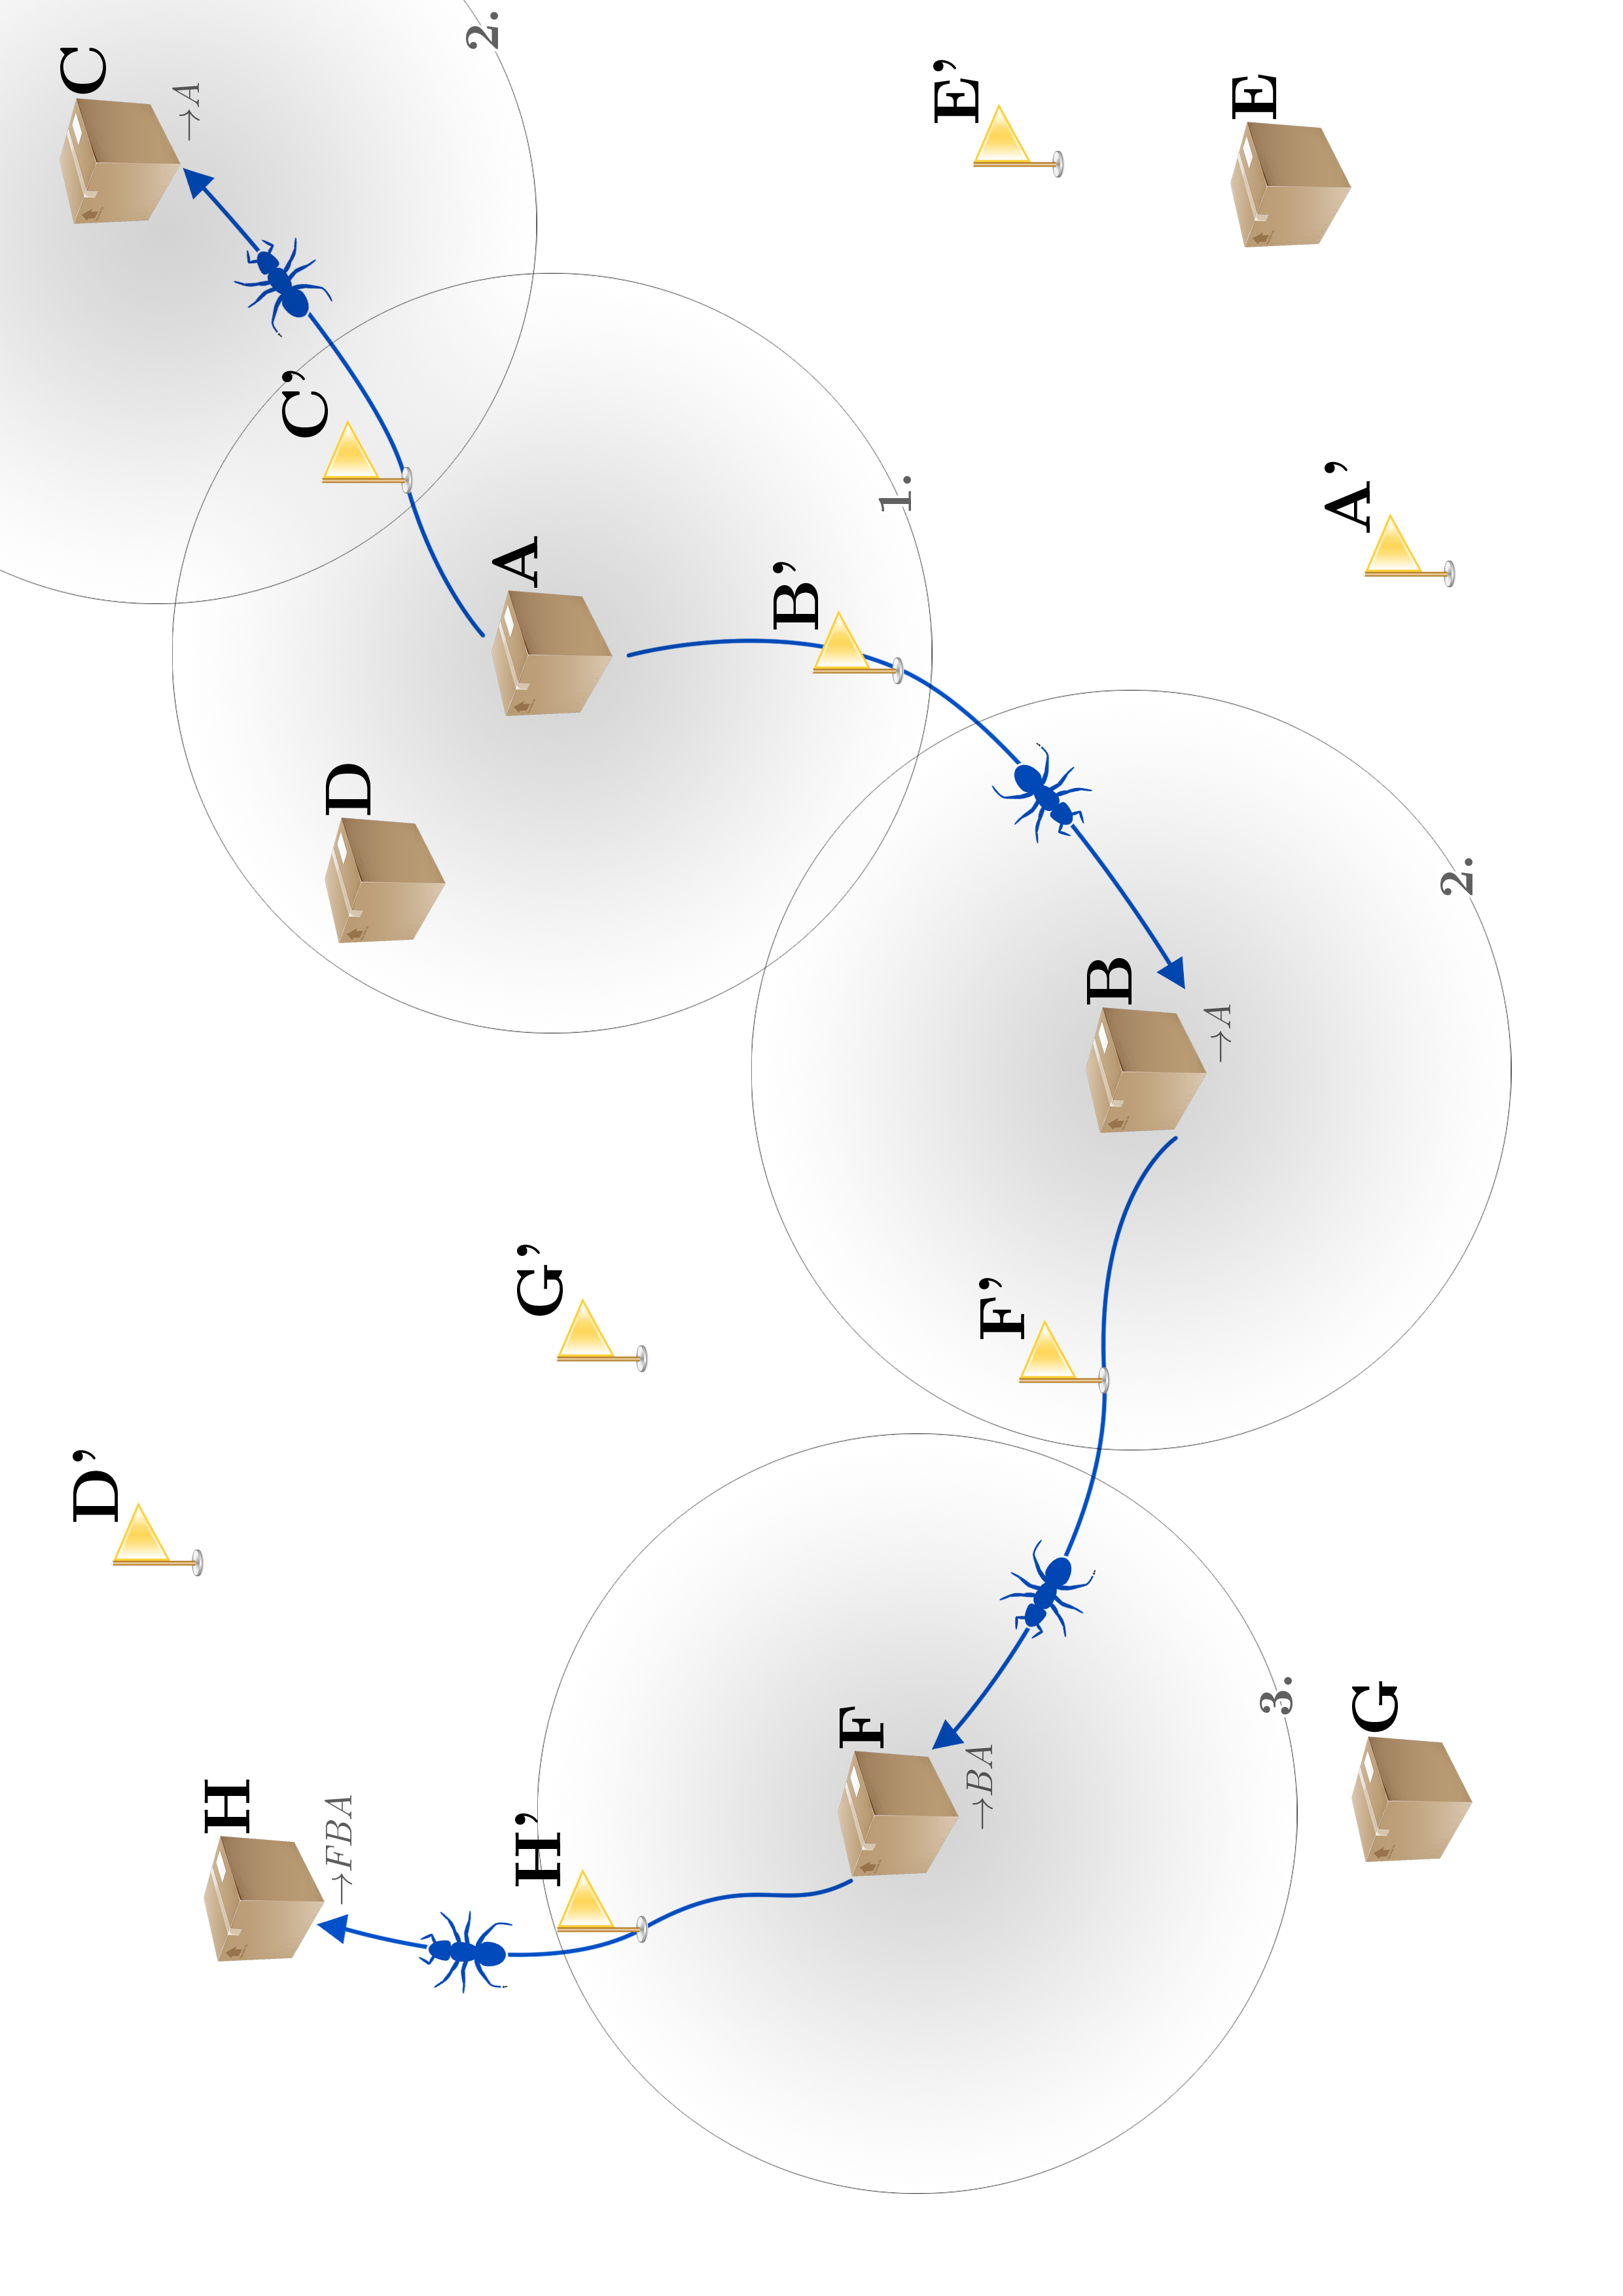
\includegraphics[width = 0.90\textwidth]{./figs/feasibility.png}}
		\end{center}
		\caption{Scenario I (\ref{subsec:scenario1})}
		\label{Fig:scenario1}
        \vspace{0.5pt}
\end{figure}

\begin{figure}[!h]
        \vspace{0.5pt}
        \begin{center}
       			\setlength\fboxsep{0.5pt}
				\setlength\fboxrule{0.5pt}
                \fbox{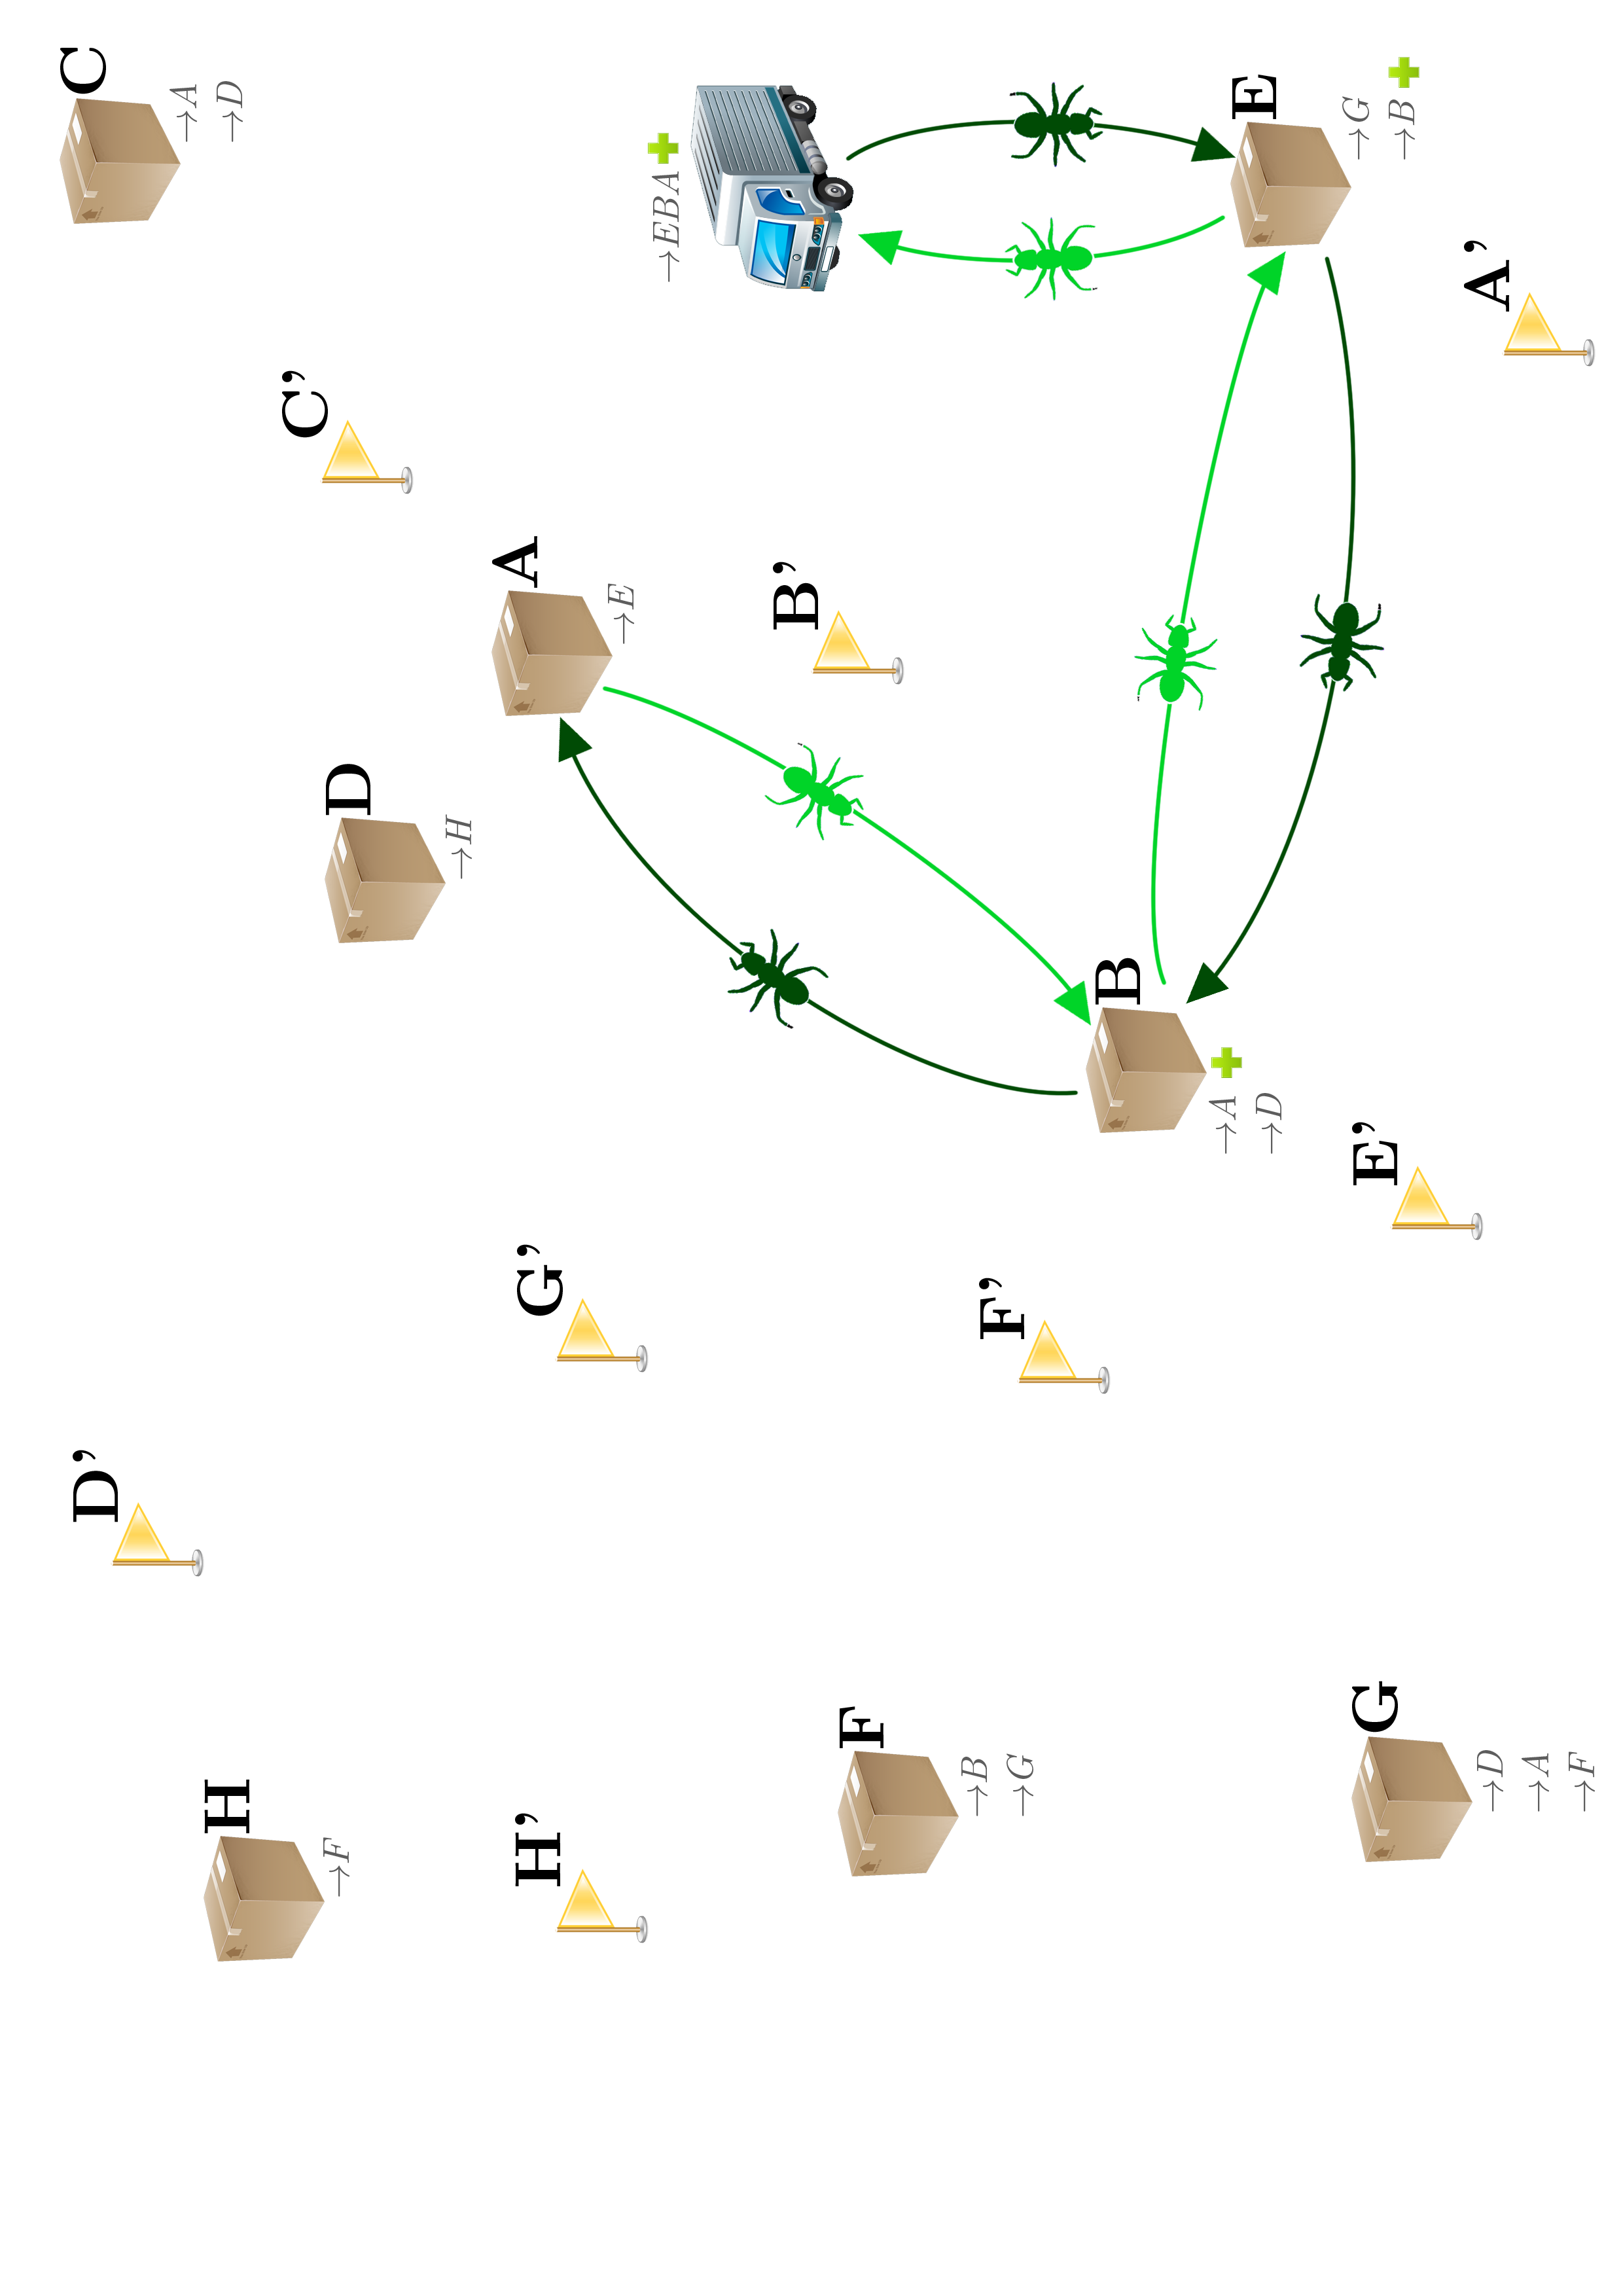
\includegraphics[width = 0.90\textwidth]{./figs/exploration.png}}
		\end{center}
		\caption{Scenario II (\ref{subsec:scenario2})}
		\label{Fig:scenario2}
        \vspace{0.5pt}
\end{figure}

\begin{figure}[!h]
        \vspace{0.5pt}
        \begin{center}
       			\setlength\fboxsep{0.5pt}
				\setlength\fboxrule{0.5pt}
                \fbox{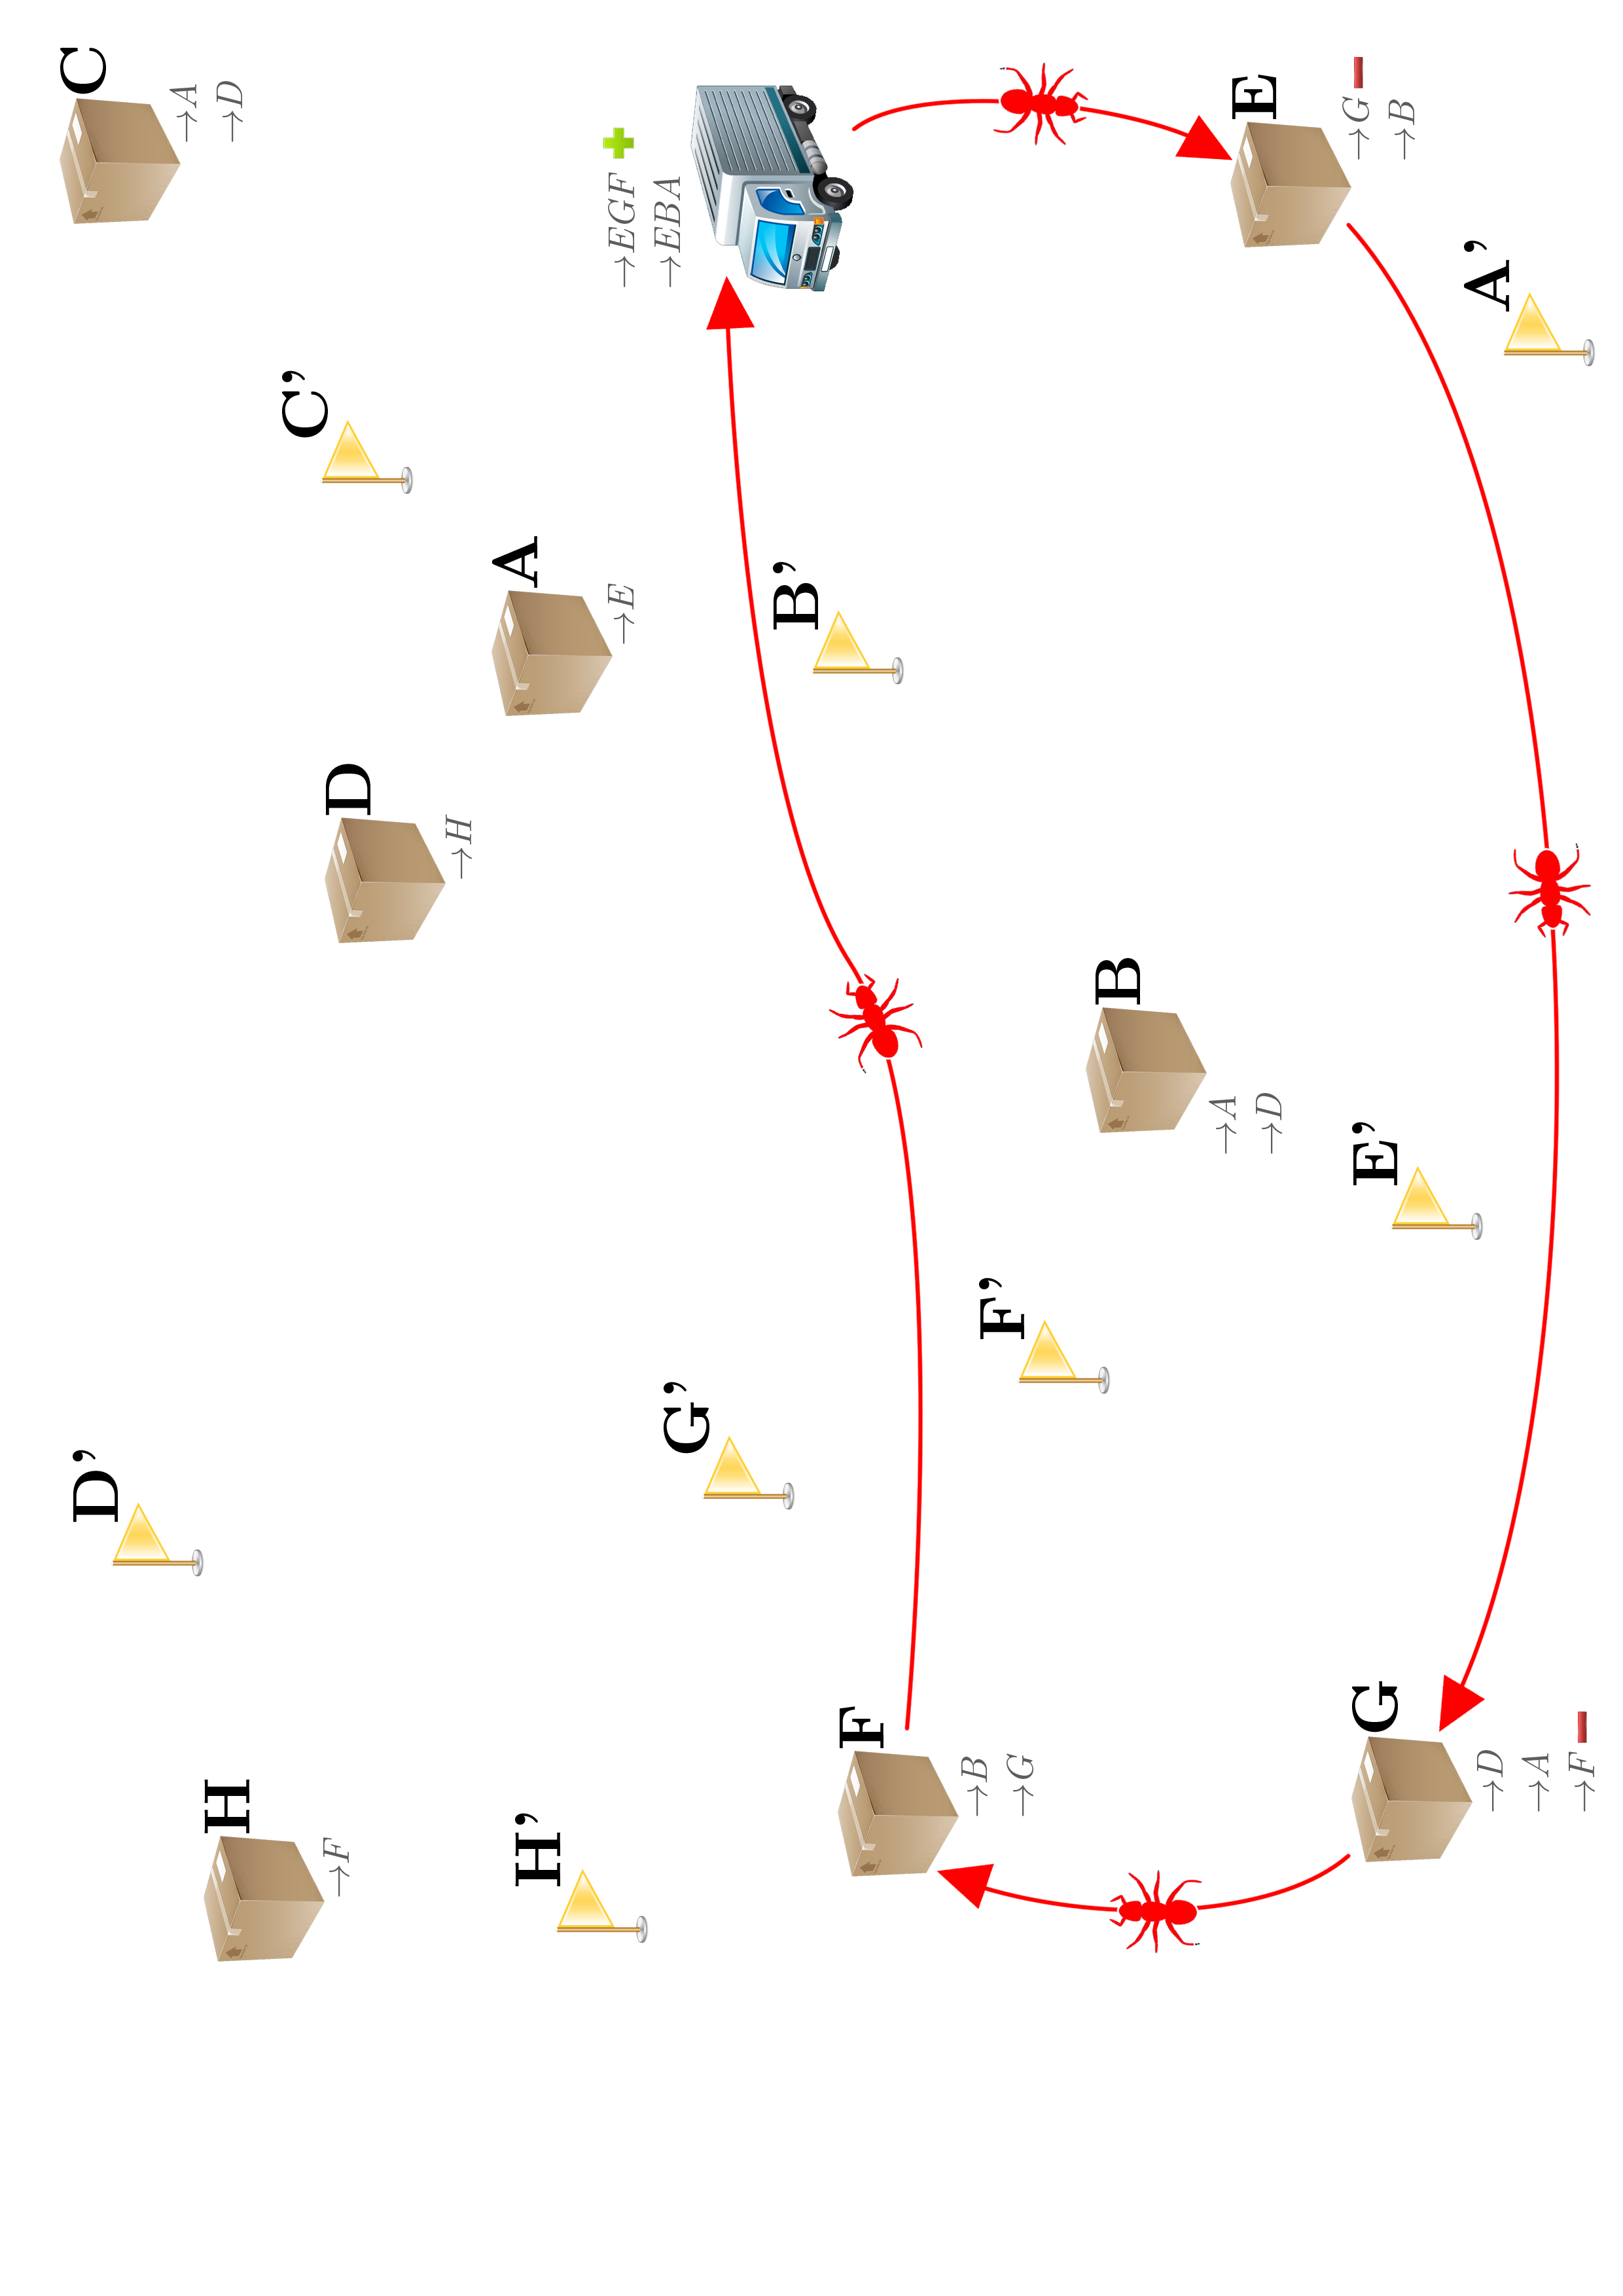
\includegraphics[width = 0.90\textwidth]{./figs/intention.png}}
		\end{center}
		\caption{Scenario III (\ref{subsec:scenario3})}
		\label{Fig:scenario3}
        \vspace{0.5pt}
\end{figure}
